\documentclass{standalone}
\usepackage[dvipsnames,svgnames,x11names]{xcolor}
\usepackage{tikz}
\usepackage{pgfplots}
\pgfplotsset{compat = 1.12}
\usepackage{../thesismath}
\begin{document}
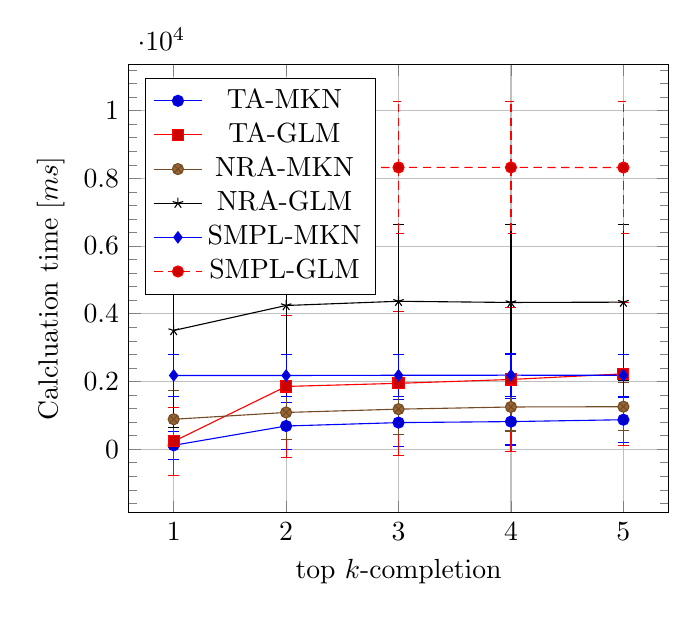
\begin{tikzpicture}[baseline]

\begin{axis}[
  xlabel = {top $k$-completion},
  xtick = {1, ..., 5},
  ylabel = {Calcluation time [$m s$]},
  minor y tick num = 4,
  grid = major,
  legend entries = {{TA-MKN}, {TA-GLM}, {NRA-MKN}, {NRA-GLM}, {SMPL-MKN}, {SMPL-GLM}},
  legend pos = north west,
]

% over 100 test sequences on my own machine

% TA-MKN
\addplot+[
  error bars/.cd,
  y dir = both,
  y explicit,
] table [y error = us_error] {
  n us       us_error
  1  114.599  419.357
  2  684.568  705.912
  3  785.033  695.001
  4  814.756  692.720
  5  870.166  670.989
};

% TA-GLM
\addplot+[
  error bars/.cd,
  y dir = both,
  y explicit,
] table [y error = us_error] {
  n us       us_error
  1  229.566  996.888
  2 1853.806 2108.055
  3 1945.700 2125.902
  4 2059.329 2119.993
  5 2225.788 2115.173
};

% NRA-MKN
\addplot+[
  error bars/.cd,
  y dir = both,
  y explicit,
] table [y error = us_error] {
  n us       us_error
  1  883.680  844.083
  2 1085.228  787.949
  3 1182.359  746.578
  4 1246.696  708.485
  5 1254.554  707.658
};

% NRA-GLM
\addplot+[
  error bars/.cd,
  y dir = both,
  y explicit,
] table [y error = us_error] {
  n us       us_error
  1 3506.086 2871.907
  2 4244.655 2402.179
  3 4369.192 2266.325
  4 4333.634 2297.886
  5 4343.249 2300.984
};

% SMPL-MKN
\addplot+[
  error bars/.cd,
  y dir = both,
  y explicit,
] table [y error = us_error] {
  n us       us_error
  1 2178.157  625.296
  2 2176.596  626.603
  3 2183.488  625.449
  4 2185.850  624.627
  5 2182.684  625.372
};

% SMPL-GLM
\addplot+[
  error bars/.cd,
  y dir = both,
  y explicit,
] table [y error = us_error] {
  n us       us_error
  1 8315.938 1941.474
  2 8313.401 1943.088
  3 8322.613 1945.171
  4 8323.701 1945.066
  5 8320.141 1944.259
};

\end{axis}

\end{tikzpicture}
\end{document}
